% !TEX root = ../my-thesis.tex
%
\chapter{Introduzione}
\label{sec:intro}
\cleanchapterquote{The Semantic Web is not a separate Web but an extension of the current one, in which information is given well-defined meaning, better enabling
computers and people to work in cooperation.}{Tim Berners-Lee}{}

Il Web, nei suoi quasi 30 anni di vita, si è evoluto da semplice archivio di documenti ipertestuali a base di conoscenza eterogenea. Questo cambiamento è stato graduale e non ha stravolto la struttura originaria del Web. Open Data e Semantic Web sono stati i due movimenti che hanno consentito congiuntamente la crescita di un Internet in cui uomini e macchine possono collaborare in maniera più efficace. Il contenuto Web è stato strutturato, arricchito da metadati, identificato univocamente, e collegato formando quelli che oggi vengono chiamati Linked Data.

Quello della generazione di Linked Data è un processo ancora in corso e che sta coinvolgendo sempre più organizzazioni, principalmente di tipo governativo, alimentando il concetto di Open Government. Sono stati  quindi delineati degli standard di creazione e distribuzione di Linked Data. 

Rendendo disponibili al pubblico dati che prima erano centralizzati e privati e donandogli una struttura interrogabile sia dall'intelligenza umana che da quella artificiale, cominciano a svilupparsi nuovi servizi in ambito culturale, scientifico, economico e governativo, permettendo partecipazione, trasparenza e condivisione.

In questo capitolo viene descritto come e perché il Web è evoluto in questa direzione, quali sono stati gli interessi e i precursori di questo cambiamento, come e da chi vengono prodotti oggi i Linked Open Data e quali sono i risultati e le sfide attuali.



\section{Storia del (Semantic) Web}
\label{sec:intro:web_history}

 
Il 6 Agosto 1991, presso il CERN, Tim Berners-Lee pubblica il primo sito web e mette a disposizione delle persone un innovativo e semplice mezzo di condivisione delle informazioni. 

Inizialmente il Web è stato usato in maniera molto semplice come grande archivio globale di documenti ipertestuali.
Il sistema di navigazione del web non forniva molte alternative: partendo da una risorsa documentale nota la si esplorava, tramite link, in cerca di nuove informazioni. 

In seguito l'indicizzazione degli indirizzi e la creazione dei motori di ricerca hanno introdotto la possibilità di interrogare la rete Internet e di cercare le informazioni in base a delle parole chiave. Tuttavia, pur avendo di molto ampliato le possibilità e il numero di utenti che ogni giorno utilizzano un browser, il tipo di interazione tra umano e macchina è rimasto ben diverso da quello tra persone.

Con l'avvento di database e linguaggi di programmazione Web, le informazioni digitali hanno cominciato a proliferare sia in ambito commerciale che di ricerca scientifica e ad adattarsi dinamicamente ad esigenze e comportamenti  dell'utente. 

Prima di proseguire è necessario marcare una linea di separazione tra i concetti di \textit{contenuto} o \textit{documento} e quello di \textit{dato}; adottando un’immagine proposta da Tim Berners-Lee, possiamo affermare che il contenuto è qualcosa che possiamo semplicemente leggere, mentre un dato può essere processato in differenti modi per creare nuova informazione.

I contenuti, pur provenendo molto spesso da basi strutturate di dati, hanno mantenuto per molto tempo l'esclusiva finalità di essere consultati dai soli utenti, rimanendo non processabili per le macchine. I dati invece hanno continuato ad avere le limitazioni di essere:
\begin{enumerate}
\item interrogabili dagli utenti finali esclusivamente tramite query predefinite dai progettisti e fornite sotto forma di interfacce web (form di ricerca),
\item centralizzati,
\item vincolati da licenze e diritti di autore,
\item scollegati da altri dati di altre fonti.
\end{enumerate}
Per combattere queste limitazioni, l'idea di accesso e riutilizzo libero e aperto che per tempo era stata associata al software (Open Source) è stata estesa al concetto di dato in generale, portando alla nascita del movimento Open Data.
Spesso i dati sono controllati da organizzazioni, sia pubbliche che private, che non ne consentono la consultazione e il riutilizzo. I sostenitori dell'idea di Open Data promuovono la cessazione di ogni limitazione di accesso a qualsiasi forma di dato, supportando una totale apertura. In particolare una delle organizzazioni internazionali di riferimento per il movimento, la \textit{Open Knowledge Foundation} \cite{okfn}, definisce gli Open Data e Open Content come: "dati e contenuti che possono essere liberamente usati, modificati e condivisi da chiunque e per qualsiasi motivo". Questo pensiero viene sempre di più assecondato e alimentato da enti governativi nazionali e internazionali, permettendo progressi in ambito culturale, scientifico, economico, ambientale e finanziario. 

Come Internet ha permesso la nascita del Web, gli Open Data hanno fornito l'infrastruttura perfetta per i Linked Data. Open Data ha reso i dati decentralizzati e accessibili a tutti, ma per arrivare ad un sistema di interrogazione potente e automatizzabile è necessario un ulteriore sviluppo. Proprio da colui che il Web l'ha inventato nasce la sua evoluzione: il \textit{Semantic Web} \cite{10.2307/26059207}\cite{semantic_web}\cite{Bizer2009LinkedD}\cite{BernersLee2006TabulatorEA}\cite{semantic_web_w3c}.
Il movimento per il Semantic Web è interessato a compiere questo processo di trasformazione del documento in dato, trasformando il Web da archivio documentale a database distribuito.
Per far funzionare il Semantic Web, i computer devono avere accesso a collezioni strutturate di informazioni e insiemi di regole di inferenza per condurre deduzioni automatiche. I ricercatori di Intelligenza Artificiale hanno studiato per anni questa tecnologia denominata \textit{rappresentazione della conoscenza}, anche prima della nascita del Web. L'ambizione è quella di stimolare le organizzazioni mondiali di ogni genere a contribuire alla costruzione di una base di conoscenza condivisa, sia per le persone che per i computer, al fine di favorire la qualità della loro cooperazione.
Il contenuto di un documento Web moderno, pur provenendo da fonti strutturate come database, perde il suo significato semantico e relazionale intrinseco nel momento in cui viene espresso sotto forma di documento HTML. Per valorizzare il dato è importante che esso:

\begin{itemize}
\item abbia una struttura standard,
\item venga corredato da metadati standard,
\item sia identificabile,
\item sia collegato ad altri dati.
\end{itemize}

Gli sforzi provenienti dai movimenti Open Data e Semantic Web si fondono così sotto il nome di Linked Open Data. Tim Berners-Lee formula una classificazione a "5 stelle" per gli Open Data, in cui il livello Linked è proprio quello più avanzato \cite{5_star_open_data}. I primi tre livelli definiscono gli Open Data come:
\begin{enumerate}
\item accessibili in rete,
\item comprensibili da un calcolatore,
\item in un formato non proprietario.
\end{enumerate}
Gli ultimi due livelli invece stabiliscono che per essere Linked, un dato deve essere inoltre nel formato standard prestabilito \textit{RDF} e collegato ad altre risorse. Un dato isolato possiede poco valore, ma se "linkato" ad altri dati assume nuovi significati deducibili dal grafo di dati a cui è connesso.

\begin{figure}[htb]
	\fbox{\includegraphics[width=\textwidth]{gfx/web_timeline.pdf}}
	\caption{Web timeline}
	\label{fig:introduction:web_timeline}
\end{figure}


Per capire le potenzialità del Web Semantico basta pensare a un episodio che è probabile vivere nell'interazione con un motore di ricerca: fare richieste basate sul significato invece che sulle parole chiave del tipo "Chi è l'inventore del Web?". Una simile interrogazione avrebbe prodotto in passato risultati tutt'altro che precisi, richiedendo la lettura all'interno dei documenti restituiti come risultato o la formulazione di una nuova ricerca. Il motivo era dovuto alla mancanza di struttura semantica nei documenti HTML indicizzati dai motori di ricerca.
Quello che invece otteniamo oggi è proprio la risposta "Tim Berners-Lee" (Fig. \ref{fig:introduction:ricerca_semantica}), come se il nostro interlocutore fosse una persona informata sulla storia del Web.

\begin{figure}[htb]
	\fbox{\includegraphics[width=\textwidth]{gfx/ricerca_semantica.pdf}}
	\caption{Ricerca semantica}
	\label{fig:introduction:ricerca_semantica}
\end{figure}

Questo risultato che può sembrare irrilevante all'utente meno fantasioso, è in realtà di incredibile importanza ed è frutto di un meccanismo di inferenza che coinvolge Linked Data e Intelligenza Artificiale. Tale logica è estendibile, per esempio, a insiemi di dati di rilevanza nell'ambito della ricerca e provenienti da fonti diverse, trasformando dati che prima erano slegati e strutturati secondo la logica decisa dalla fonte (e quindi interrogabili solo avendone diritto d'accesso e conoscendo la struttura specifica), in dati collegati e interrogabili con un processo di inferenza semantica affine a quello della mente umana.

Il meccanismo di interrogazione si evolve da semplice ricerca di termini chiave a qualcosa di più elaborato. Il linguaggio naturale della query viene analizzato con tecniche di \textit{NLP (Natural Language Processing)}, scomponendone il testo, definito in ambito linguistico come proposizione, nella sua struttura fondamentale "soggetto-predicato-oggetto". Nel caso della domanda precedente, il soggetto è l'incognita che l'utente vuole conoscere, il predicato è "essere inventore" e l'oggetto è "il Web".
Immaginiamo ora una base di conoscenza in cui i dati siano strutturati considerando come modello proprio la proposizione. Per dare una risposta alla domanda, sarebbe sufficiente trovare tutte le triple "soggetto-predicato-oggetto" che abbiano predicato e oggetto come sopra e restituire come risultato ciascun soggetto. Ebbene questo formato è proprio lo standard del Semantic Web e dei Linked Data: RDF. 

\section{Struttura standard del Semantic Web}
\label{sec:intro:web_history}

Il modello \textbf{\textit{RDF}} (\textit{Resource Description Framework})\cite{rdf_overview}, rappresenta l'informazione in maniera simile a come viene espressa dalla logica umana, sotto forma di asserzioni (o proposizioni) composte da \textit{soggetto}, \textit{predicato} e \textit{oggetto}. Il modello RDF viene serializzato in diversi tipi di formato che non ne alterano la logica e sono intercambiabili. I formati più popolari per la serializzazione di modelli RDF sono: \textit{RDF/XML, Turtle, NTriples}.

Il lettore più scrupoloso avrà certamente obiettato, nella scorsa sezione, che il linguaggio naturale è per natura ambiguo e quindi inadatto ad un processo di inferenza. Per questo motivo, nella progettazione delle basi di conoscenza Linked Data, si è scelto di usare come classe di dato fondamentale quella che viene chiamata \textit{entità} o \textit{nodo}. Tali entità possono essere usate come soggetto e oggetto di una tripla. Per essere distinte in maniera non ambigua vengono etichettate con degli \textit{\textbf{URI} (Universal Resource Identifier)}. 
Queste entità rappresentano qualsiasi concetto del mondo reale. 
Dato che gli RDF usano URI per codificare le informazioni, ci si assicura che i concetti non siano solo parole in un documento, ma che siano unicamente identificati, referenziabili da altre risorse e disponibili nel Web (nel caso in cui un URI sia specializzato in un URL HTTP). 


\iffalse
\begin{figure}[htb]
	
   \fbox{ includegraphics[width=\textwidth]{gfx/LOV.pdf} }
	\caption{Grafo Linked Open Vocabularies (Ontologie)}
    {Mostra tutte le ontologie OWL esistenti}
    {(\textit{Linking Open Data cloud diagram 2017, by Andrejs Abele, John P. McCrae, Paul Buitelaar, Anja Jentzsch and Richard Cyganiak. http://lod-cloud.net/})}
	\label{fig:introduction:lov}
\end{figure}
\fi

Come già detto, i dati presenti in un database sono strutturati, ma fare Linked Open Data non significa solamente diffondere tali dati pubblicamente, ma farlo utilizzando una struttura e dei significati (metadati) condivisi da tutti. Se il problema di avere una struttura standard viene risolto dall'uso dell'RDF, quello di fornire tipi di metadati standard, dare significato e definire regole di inferenza viene assolto dalle \textit{ontologie} (o \textit{vocabolari}) \textit{OWL} \cite{w3c_owl}. 

Invece di utilizzare nomi di \textit{proprietà} (\textit{predicati} o \textit{relazioni}) diversi per lo stesso concetto, la comunità scientifica lavora alla definizione di insiemi di proprietà per tipi di concetti diversi. E' così che anche l'ambiguità di descrivere la stessa proprietà con parole diverse viene superata utilizzando predicati creati appositamente da organizzazioni autorevoli, identificati da URI e non ripetuti. Un'ontologia è, in altre parole, una tassonomia che esprime il significato semantico e le relazioni di una categoria omogenea di dati.

Ricapitolando, i Linked Data sono composti da due insiemi di dati etichettati da URI: le \textit{entità} (o \textit{nodi}) e le \textit{proprietà} (o \textit{predicati}). Coppie di entità possono essere relazionate tra loro dalle proprietà. 

Esistono anche delle entità speciali che non sono identificate da 
URI: \nolinebreak
\begin{itemize}
\item \textit{Literal}: dati primitivi testuali come numeri, date o nomi propri.
\item \textit{Blank Nodes}: nodi anonimi usati solitamente come nodi strutturali ausiliari di nodi complessi.
\end{itemize}

Formalmente \cite{RDF_DEFINITION} un RDF è definito come una raccolta di triple. Un insieme di tali triple è definito \textit{Grafo RDF}. 
Una \textit{tripla RDF} contiene tre componenti ordinate:
\begin{enumerate}
\item il \textit{soggetto}, che è un \textit{URI RDF} o un \textit{Blank node};
\item il \textit{predicato} (o \textit{proprietà}) che è un \textit{URI RDF} (definito in un'ontologia);
\item l'\textit{oggetto} che è un \textit{URI RDF} o un \textit{Blank node} o un \textit{Literal}.
\end{enumerate}
Per convenzione ci si riferisce ad una tripla RDF con la notazione \textit{(s, p, o)}.
\begin{figure}[htb]
	\fbox{\includegraphics[width=\textwidth]{gfx/rdf_triple_example.pdf}}  
	\caption{Tripla RDF}
	\label{fig:introduction:rdf_triple}
\end{figure}



A livello intuitivo una tripla può essere illustrato da un grafo orientato in cui ogni tripla soggetto-predicato-oggetto è rappresentata come nodo-arco-nodo  (Fig. \ref{fig:introduction:rdf_triple}). L'intero database globale di Linked Data può essere visto come una grande tabella di tre colonne oppure come un grande grafo (Fig. \ref{fig:introduction:lod}).
Si noti che i literal possono comparire solamente come oggetto delle triple e quindi come nodi foglia del grafo.

\begin{figure}[htb]
	\fbox{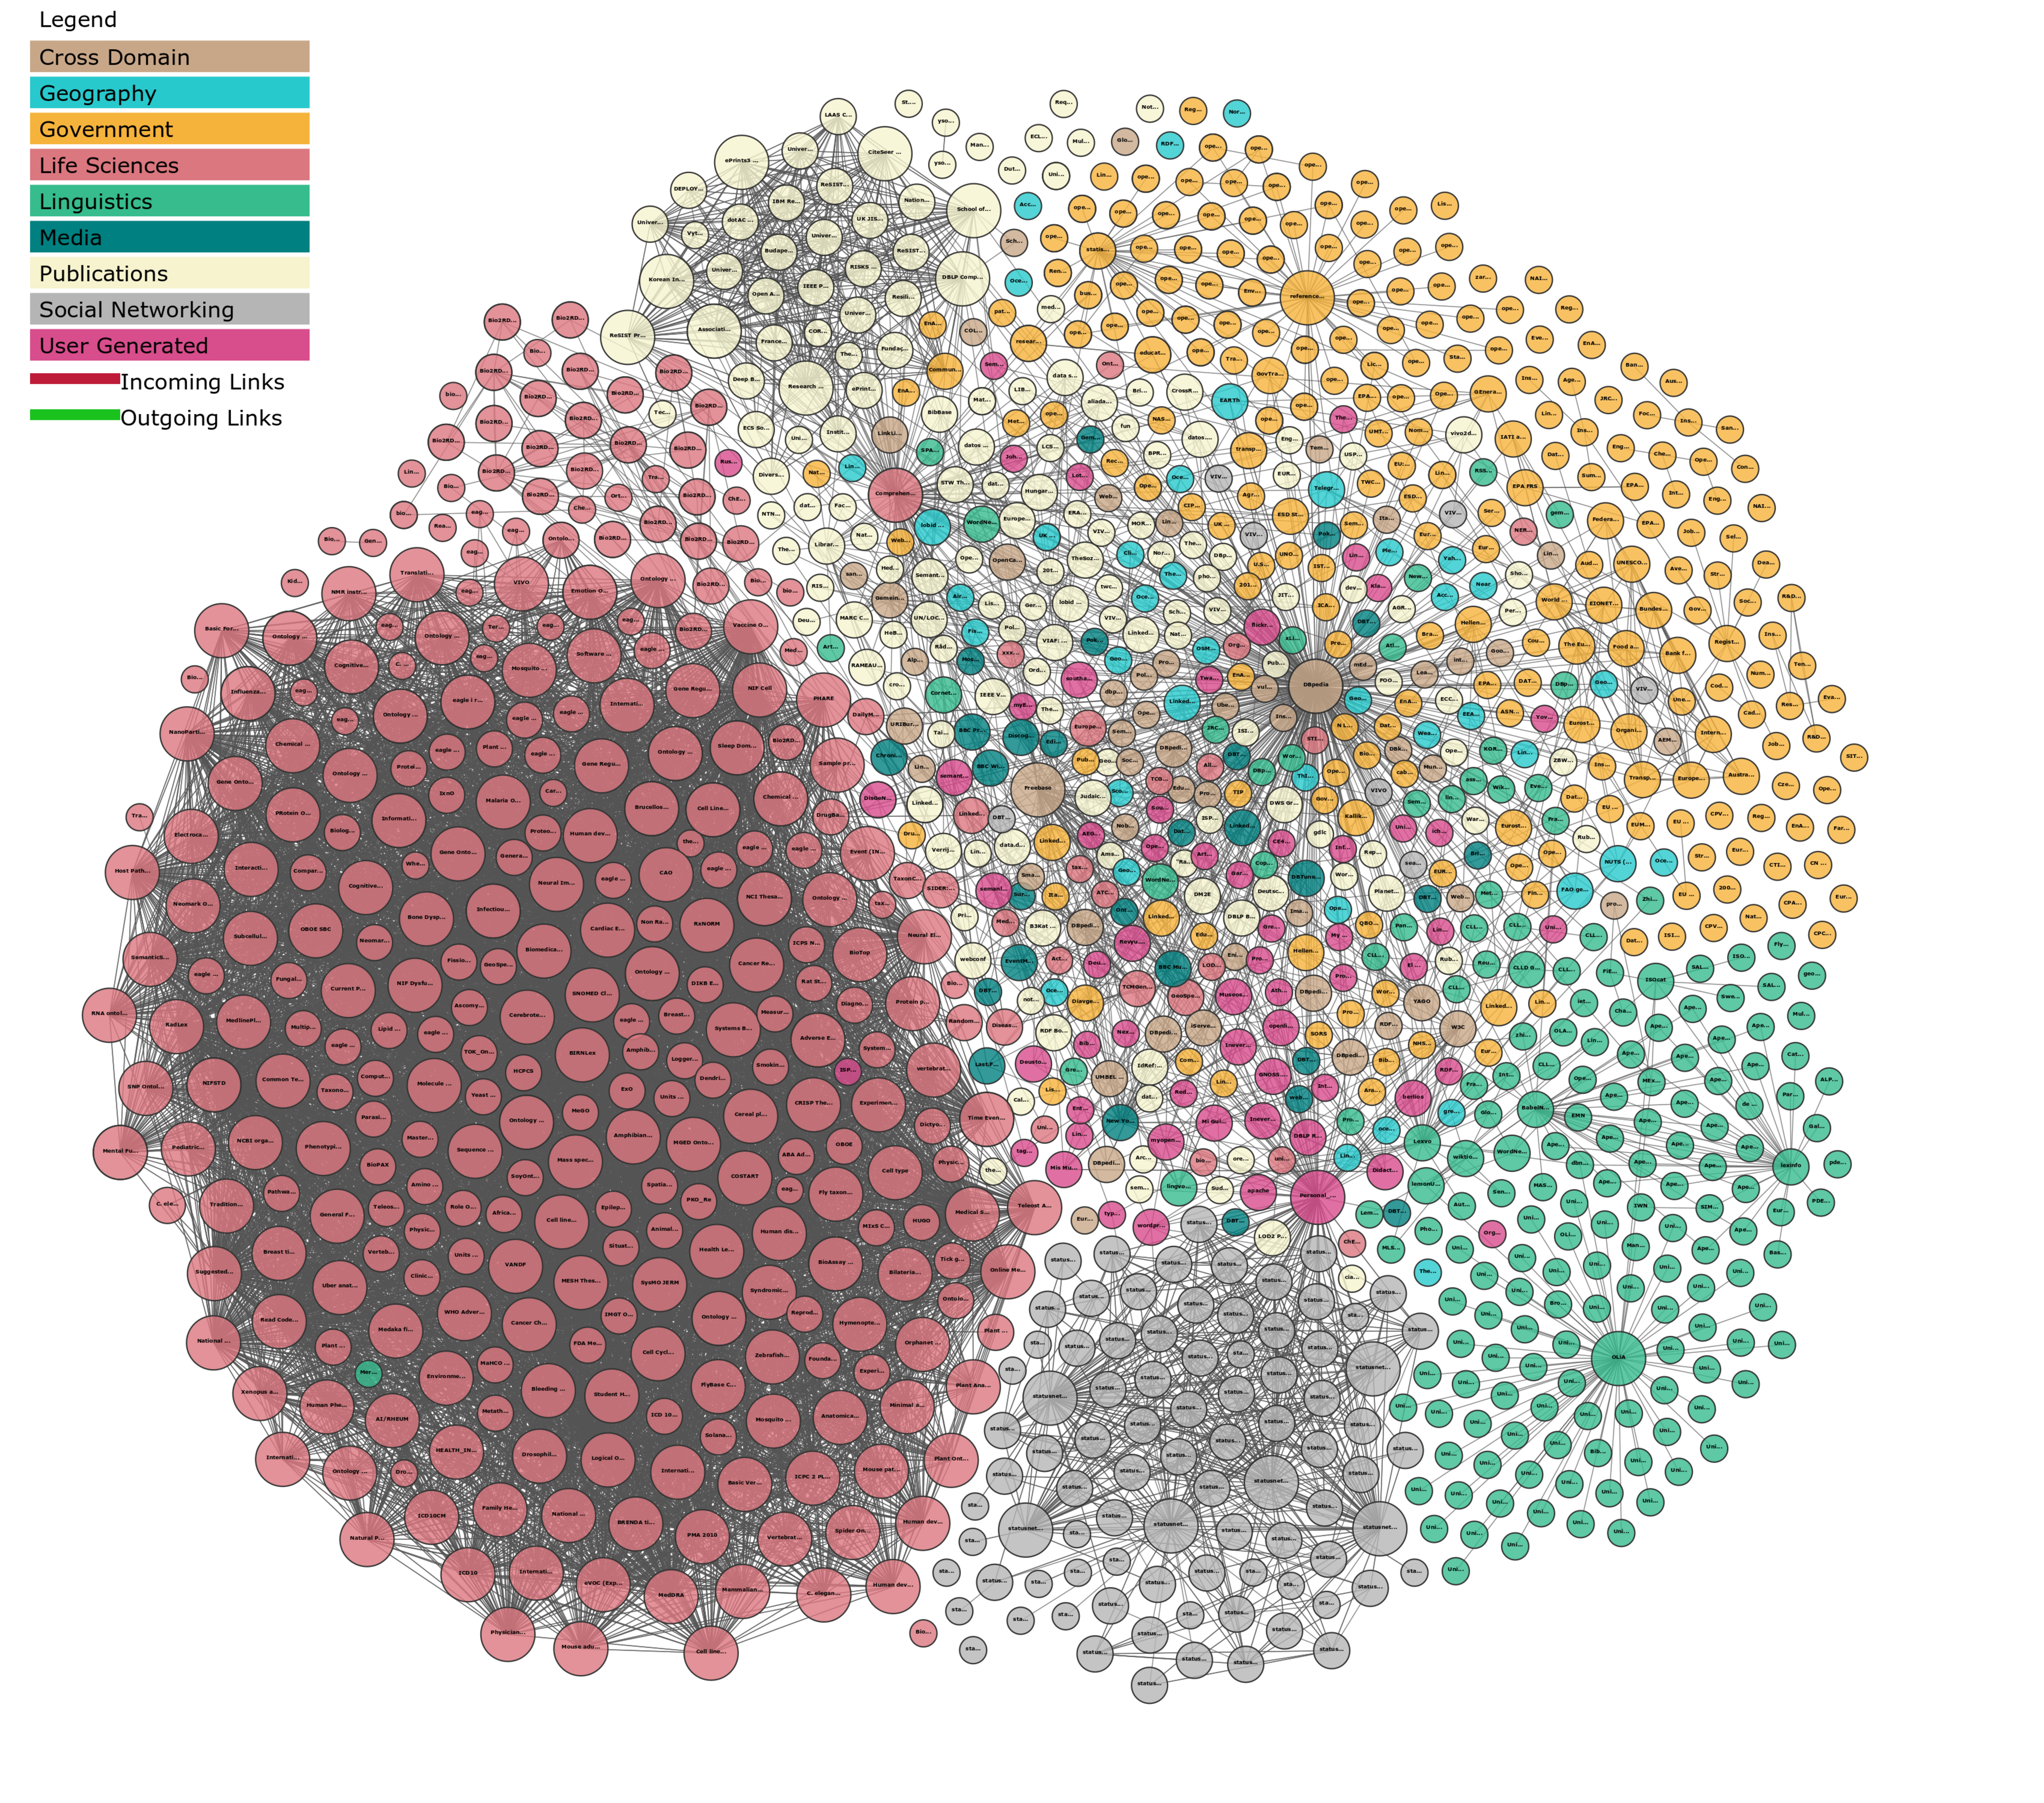
\includegraphics[width=\textwidth]{gfx/lod.pdf} }
	\caption{Grafo Linked Opend Data}
	\label{fig:introduction:lod}
\end{figure}


Come spiegato in precedenza, il fine di quanto descritto finora è quello di sviluppare un sistema che consenta una migliore interoperabilità tra programmi e persone e tra programmi ed altri programmi. Costruire quindi un sistema che cataloghi con una struttura condivisa (RDF) tutta la conoscenza umana, ne delinei la semantica e le regole di inferenza per le intelligenze artificiali (OWL) e la renda interrogabile (SPARQL). 


Così come RDF è il formato strutturale standard per il Semantic Web, \textbf{\textit{SPARQL}} (\textit{Simple Protocol And RDF Query Language}) \cite{sparql_overview} è un insieme di specifiche standard che definisce:
\begin{itemize}
\item il linguaggio di interrogazione e aggiornamento \textit{SPARQL Query/Update Language} ;
\item la struttura \textit{graph store}  in cui i dati RDF sono organizzati in sottografi identificati da URI;
\item il protocollo \textit{SPARQL Protocol} che definisce il motore di interrogazione e le comunicazioni \textit{SPARQL Graph Store HTTP Protocol}.
\end{itemize}
Questi servizi vengono resi accessibili al pubblico sotto forma di interfaccia Web e servizio REST in quello che viene definito \textit{SPARQL Endpoint}.
Il linguaggio SPARQL consente di effettuare interrogazioni che vanno dalla semplice corrispondenza di pattern su grafi, a query complesse usando operatori comuni ai linguaggi relazionali. 
Fare una interrogazione in SPARQL vuol dire navigare il grafo lungo gli archi ed i nodi fino a soddisfare tutti i vincoli dell’inferenza e restituire il grafo attraversato. Le richieste vengono serializzate mediante il formato \textit{Turtle}, mentre il risultato della richiesta può essere una tabella in diversi formati (JSON, HTML, XML, CVS) o un sotto-grafo.

L'utilizzo di proprietà, definite nelle ontologie, nella costruzione dei Linked Data, rendono l'interrogazione SPARQL in grado di effettuare l'inferenza di proprietà non esplicitamente espresse dalle entità (Esempio in figura \ref{fig:introduction:rdf_graph}).

La specifica \textit{SPARQL Federated Query} consente l'interrogazione dell'intero grafo globale avendo come unico punto di accesso un singolo SPARQL Endpoint.


\begin{figure}[htb]
\begin{tikzpicture}[node distance=2.75cm,>=stealth']
\node[vertex style=Turquoise] (Rk) {dbr:Zinédine Zidane};

\node[vertex style=BurntOrange, above of=Rk,xshift=15.5em, yshift=3.5em] (BD) {dbr:Real\_Madrid\_C.F.}
 edge [<-,cyan!60!blue] node[text style]{dbo:team} (Rk);

\node[vertex style=BurntOrange, right=2.5cm of Rk,yshift=4ex] (AP) {dbr:Juventus\_F.C.}
 edge [<-,cyan!60!blue] node[text style]{dbo:team} (Rk); 

\node[vertex style=red, below right of=Rk,xshift=9em, yshift=-6em] (JA) {dbr:Midfielder}
 edge [<-,cyan!60!blue] node[text style]{dbo:position} (Rk); 

 \node[vertex style=BurntOrange, right=2.0cm of Rk,yshift=-4em] (RN) {dbr:FC\_Girondins\_de\_Bordeaux}
 edge [<-,cyan!60!blue] node[text style]{dbo:team} (Rk); 

\node[vertex style=MidnightBlue, above left of=Rk,xshift=2em, yshift=4em] (Dr) {"Zinedine Zidane"@en}
 edge [<-,cyan!60!blue] node[text style]{rdfs:label} (Rk); 

\node[vertex style=Maroon, below of=Rk,xshift=-2em] (Skf) {dbo:Athlete}
 edge [<-,cyan!60!blue] node[text style]{rdf:type} (Rk);

\node[vertex style=Maroon, below right of=Skf, yshift=-4em] (Cf) {dbo:Person}
 edge [<-,cyan!60!blue] node[text style]{rdfs:subClassOf} (Skf);

\begin{pgfonlayer}{background}
\draw[Maroon,fill=Maroon,dashed,fill opacity=0.1](Rk.north) 
to[closed,curve through={(Rk.north west).. (Rk.west) .. (Rk.south west) 
..($(Rk.south west)!0.5!(Skf.north)$) .. (Skf.north     west).. (Skf.west) 
.. (Skf.south west) .. ($(Skf.south)!0.75!(Cf.west)$) .. (Cf.west) 
.. (Cf.south west) .. (Cf.south) .. (Cf.south east) .. (Cf.east) 
.. ($(Cf.north east)!0.65!(Skf.south east)$) .. (Skf.east) 
.. (Skf.north east).. ($(Skf.north)!0.35!(Rk.south east)$) 
.. (Rk.south east) .. (Rk.east)..(Rk.north east)}](Rk.north);
\end{pgfonlayer}

\end{tikzpicture}
	\caption{Inferenza SPARQL}{L'area con sfondo marrone indica un passo di inferenza. Il tipo \textit{Person}, può essere dedotto dal tipo \textit{Athlete} direttamente collegato all'entità RDF presa in considerazione}
	\label{fig:introduction:rdf_graph}
\end{figure}

\section{Creazione e pubblicazione dei Linked Data}
\label{sec:intro:linked_data_production}

Sarebbe auspicabile che tutte le organizzazioni mondiali seguissero le indicazioni della comunità per il Semantic Web permettendo la costruzione di basi di conoscenza più complete e servizi, che le sfruttano, sempre più avanzati. A maggior ragione, il cittadino dovrebbe pretendere che questo avvenga per quelle organizzazioni che sono di origine pubblica. Questa legittima pretesa ha dato origine all'idea di \textit{Open government} che, in linea con il movimento open in generale, cerca di rendere il lavoro dei governi trasparente, responsabile, comprensivo e partecipativo per il cittadino. Come conseguenza a questa esigenza e opportunità, organizzazioni governative (come AGID in Italia) e non (Open Knowledge International) si sono attivate per il perseguimento delle politiche Open Data, elaborando linee guida e fornendo risorse di supporto.

Linee guida per la pubblicazione di Open Data a livello Linked sono state formulate da Tim Berners-Lee\cite{5_star_open_data} sotto forma di quattro semplici regole:
\begin{enumerate}
\item usare gli URI per identificare i dati;
\item usare URI HTTP (URL) in modo che le persone possano "visitare" questi dati usando un semplice browser;
\item le risorse identificate da URI devono fornire informazioni utili utilizzando gli standard RDF e SPARQL;
\item includere URI che collegano i dati tra loro, in modo da estendere il sistema sul quale fare inferenza \label{sec:intro:link_discovery}.
\end{enumerate}

Un'altra buona abitudine è quella di riutilizzare il più possibile gli URI già esistenti e fare collegamenti ad altre fonti. In questo modo il grafo globale Linked Data si mantiene più connesso e meno spazioso e di conseguenza più veloce ed interessante da interrogare.
Oltre alle linee guida per la strutturazione del dato, varie organizzazioni hanno formulato specifiche per l'intero processo produttivo di Linked Open Data.

%%Nuova sezione
Per esaminare il processo di produzione dei Linked Data ci si riferisce nel resto di questa sezione al caso reale di generazione dei Linked Open Data della Regione Umbria. Esso ci consente un'analisi senza perdita di generalità in quanto svolto in conformità alle linee guida delineate dall'AGID  e in ottemperanza alla direttiva Europea 2013/37/UE, detta PSI 2.0, che impone alle pubbliche amministrazioni azioni finalizzate al riutilizzo dei dati pubblici anche per fini commerciali. 

\subsection{Linked Open Data della Regione Umbria}
\label{sec:intro:linked_data_production:RU}

La Regione Umbria ha intrapreso fin dal 2014 il percorso di apertura dei dati regionali attraverso il programma \#opendata dell’Agenda Digitale Umbra. Grazie alla collaborazione con \textit{Umbriadigitale s.c.a r.l.} e con il \textit{Dipartimento di Informatica, Sistemistica e Comunicazione dell’Università Milano Bicocca} a poco tempo dall’avvio del percorso, si è giunti a creare l’ambiente tecnico e metodologico che ha permesso di pubblicare i primi Linked Open Data nel portale regionale. Questo meccanismo di produzione e pubblicazione dei Linked Data della Regione Umbria è attualmente assolto da un progetto gestito dall'Ing. Azzurra Pantella di Umbria Digitale, a cui l'autore di questa tesi ha l'opportunità di collaborare.

La Regione Umbria segue il modello ODMC (Open Data Management Cycle) \cite{ODMC} che delinea l'intera organizzazione per la gestione di Open Data. Si tratta di un processo ciclico composto da quattro punti:
\begin{enumerate}
\item identificazione dei dataset da pubblicare, richiedendo la partecipazione diretta del cittadino alla proposta di essi;
\item analisi della disponibilità, del valore e della qualità dei dati richiesti ed eventuale pubblicazione;
\item monitoraggio delle performance dei dataset;
\item mantenimento, aggiornamento ed eventuale dismissione  dei dati pubblicati.
\end{enumerate}


Il software open source CKAN \cite{CKAN} rappresenta un elemento di centrale importanza nell'implementazione di tale modello. CKAN permette di catalogare i dataset e descriverli attraverso una serie di metadati che da un lato aiutano gli utenti a navigare tra le informazioni e dall’altro favoriscono l’indicizzazione degli stessi dataset sui motori di ricerca. Sono molti, e in continuo aumento, gli enti pubblici che hanno adottato CKAN per esporre il proprio patrimonio informativo in formato Open Data, rendendolo uno standard \textit{de facto}\cite{ckan_agid}.
Il portale \textit{dati.umbria.it }\cite{datiumbria} è il punto di accesso per il cittadino ai Linked Open Data della Regione Umbria. E' un portale costruito su CKAN ed implementa, tra l'altro, il primo punto del modello ODMC sopra esposto fornendo un form per la proposta da parte del cittadino della messa a disposizione di nuovi dataset; quelli proposti e valutati positivamente, una volta estratti e strutturati, vengono pubblicati su questa piattaforma.

Una volta superato il processo di verifica della disponibilità e attestazione di utilità del dataset, si innesca il processo di analisi del dato. I dati sorgente possono essere generalmente immagazzinati in: database, file strutturati, file non strutturati (documenti di testo libero) o documenti cartacei. Ad oggi i soli dati che vengono trasformati in Linked Data sono quelli disponibili in formato strutturato (file o database). Per i dati non strutturati non esistono ancora soluzioni in grado di fornire un processo adeguatamente rapido, automatizzato, accurato e poco dispendioso di trasformazione. Quello di estrarre informazioni strutturate da documenti non strutturati è un problema attuale a cui si cerca di dare un contributo in questo lavoro.

I dati strutturati vengono sottoposti ad un processo di ETL (Extract Transform Load) usando il framework \textit{UnifiedViews} \cite{unifiedviews}. Le basi di dati vengono denormalizzate, se 
necessario, e viene fatta una selezione delle tabelle le cui tuple siano da pubblicare. Ciascuna tupla selezionata verrà poi trasformata, alla fine del processo, in nodo RDF.

Per ogni collezione di entità selezionate si sceglie innanzitutto l'ontologia adatta a descriverle. Si selezionano come prime proprietà i predicati \textit{<http://www.w3.org/1999/02/22-rdf-syntax-ns\#type>} che identificano le classi che l'oggetto istanzia. Per esempio, per una tabella di ricercatori scientifici si potrebbe scegliere di estrarre entità del tipo \textit{<http://xmlns.com/foaf/0.1/Person>}. Di conseguenza si controllano quali proprietà della classe definita nell'ontologia è possibile soddisfare con i dati del database. Se nella tabella considerata in precedenza è presente la colonna "nome" si potrà valorizzare l'oggetto per il predicato \textit{<http://xmlns.com/foaf/spec/\#term\_firstName>}. Si ipotizzi di avere una tabella che associa i propri ricercatori con quelli di altre organizzazioni in base alle pubblicazioni che essi hanno sostenuto insieme. Se tali ricercatori hanno già una risorsa RDF che li identifica in un dataset di una fonte esterna, è possibile usare link \textit{<http://purl.org/net/soron/workPartnerOf>} che hanno come oggetto gli URI dei ricercatori esterni. Questo processo si chiama \textit{Link Discovery} ed è di fondamentale importanza per rispettare la quarta regola proposta da Tim Berners-Lee e dare valore "deducibile" ai dati pubblicati.

Al termine di questa fase di trasformazione, i dataset generati possono essere caricati sia sul catalogo CKAN che sul graph store \textit{Virtuoso Universal Server} \cite{virtuoso}. Virtuoso è un database che offre, tra le molte funzionalità, la possibilità di memorizzare, organizzare e interrogare dati RDF. Implementa quindi un motore SPARQL, e permette di organizzare i vari dataset in (sotto-)grafi identificati da URI. Il punto di accesso al motore SPARQL è un servizio REST denominato SPARQL Endpoint. 
La procedura di estrazione, trasformazione e caricamento dei Linked Data è interamente assolta da UnifiedViews definendo delle \textit{pipeline}. L'integrabilità di UnifiedViews con CKAN fa in modo che il caricamento dei dataset prodotti avvenga come un passaggio della pipeline. Lo stesso vale per Virtuoso, supportato da UnifiedViews come client. 

L'aggiornamento dei dati è reso fattibile dalla possibilità di schedulare l'esecuzione delle pipeline in UnifiedViews.

La pubblicazione dei dataset viene conclusa con l'attribuzione di una licenza open.

\section{Interrogazione dei Linked Data}
\label{sec:intro:sparql}



In questa sezione viene mostrato un caso d'uso generico dello SPARQL Query Language. Come nella sezione precedente si farà riferimento ai dati della Regione Umbria.

Il protocollo SPARQL consiste di due operazioni: \textit{query} e \textit{update}. Queste operazioni devono essere invocate e servite via HTTP GET o HTTP POST. Il punto di accesso HTTP al servizio SPARQL si chiama \textit{SPARQL Endpoint} e viene messo a disposizione del pubblico dalle organizzazioni che conservano i propri dati in un graph store. Il graph store più popolare, di cui fa uso anche la Regione Umbria, è il già citato Virtuoso. Lo SPARQL Endpoint permette a qualsiasi utente di interfacciarsi con il graph store ed interrogarne i dati e viene pubblicato per convenzione sotto il percorso \textit{"/sparql"}, nel caso specifico \textit{https://dati.umbria.it/sparql}.

Lo SPARQL Endpoint è composto da:
\begin{enumerate}
\item un input testuale per la definizione del grafo da interrogare di default (\textit{default-graph-uri}),
\item un'area testuale per l'inserimento della query,
\item un menu per la selezione del formato del risultato.
\end{enumerate}
Il meccanismo principale per calcolare il risultato delle query SPARQL è chiamato \textit{subgraph matching}.
Fare un'interrogazione in SPARQL vuol dire navigare il grafo lungo gli archi ed i nodi fino a soddisfare tutti i vincoli dell’inferenza e restituire il grafo attraversato.
Secondo questo meccanismo l'utente decide innanzitutto quali sottografi interrogare, selezionando quindi un insieme di triple RDF. Il modello della query può contenere delle variabili usate come \textit{wild cards}. Nel linguaggio SPARQL le variabili sono identificate dal simbolo "?" usato come prefisso (es. ?subject).
Il sottografo risultante deve combaciare sia con un sottografo del sottografo di partenza che con il grafo modellato dalla query.
Grazie alla struttura RDF e alle regole OWL che forniscono una interpretazione semantica per i dati, è possibile inferire nuove triple RDF implicite a partire dalle asserzioni esplicitamente dichiarate.

Come già spiegato, in un graph store i dati RDF sono organizzati in sottografi identificati da URI.
La prima cosa da fare quando si decide di interrogare un graph store che non si conosce è scoprire quali sottografi contiene. Per farlo si esegue la query in \ref{lst:intro:sparql1}, senza specificare nessun grafo di default.\\ 



\lstset{ basicstyle=\LSTfont, columns=fullflexible, xleftmargin=5mm, framexleftmargin=5mm, numbers=left, stepnumber=1, breaklines=true, breakatwhitespace=false, numberstyle=\footnotesize, numbersep=5pt, tabsize=2, frame=lines, captionpos=b}
   
\begin{lstlisting}[frame=single, caption={Individuare i grafi salvati in un graph store.},label={lst:intro:sparql1},]  
SELECT DISTINCT ?graph
WHERE{
	GRAPH ?graph {?s ?p ?o}
}
\end{lstlisting}

\begin{table}[htbp]
\begin{center}
\begin{tabular}{|l|}
\hline \textbf{?graph} \\
\hline
http://dati.umbria.it/graph/consorzi\\
\hline
http://dati.umbria.it/graph/impianti\_sportivi\\
\hline
http://dati.umbria.it/graph/attrattori\\
\hline
...\\
\hline
%table & tabelle \\
\end{tabular}
\end{center}
\caption{Risultato \textit{Snippet \ref{lst:intro:sparql1}}}
\label{tab:intro:sparql1}
\end{table}

Si sceglie poi il grafo di interesse da interrogare e si usa come grafo di default. Si procede con l'esaminare i tipi di dato contenuti nel grafo selezionato (Snippet \ref{lst:intro:sparql2}).


\begin{lstlisting}[frame=single, caption={Individuare i tipi di dato del grafo scelto.},label={lst:intro:sparql2}]  
#default-graph-uri=http://dati.umbria.it/graph/attrattori

SELECT DISTINCT ?o
WHERE{
	?s <http://www.w3.org/1999/02/22-rdf-syntax-ns#type> ?o .
}
\end{lstlisting}

\begin{table}[htbp]
\begin{center}
\begin{tabular}{|l|}
\hline \textbf{?o} \\
\hline
http://linkedgeodata.org/ontology/Attraction\\
\hline
http://dati.umbria.it/tourism/ontology/descrizione\\
\hline
http://dati.umbria.it/tourism/ontology/tempo\_di\_viaggio\\
\hline
...\\
\hline
%table & tabelle \\
\end{tabular}
\end{center}
\caption{Risultato \textit{Snippet \ref{lst:intro:sparql2}}}
\label{tab:intro:sparql2}
\end{table}

Scegliendo un tipo di dato si possono ottenere tutti i nodi del grafo che istanziano tale classe (Snippet \ref{lst:intro:sparql3}).
\begin{lstlisting}[frame=single, caption={Individuare i nodi del tipo scelto.},label={lst:intro:sparql3}]  
#default-graph-uri=default-graph-uri=http://dati.umbria.it/graph/attrattori

SELECT DISTINCT ?s 
WHERE{
    ?s  <http://www.w3.org/1999/02/22-rdf-syntax-ns#type> <http://linkedgeodata.org/ontology/Attraction> .
}
\end{lstlisting}

\begin{table}[htbp]
\begin{center}
\begin{tabular}{|l|}
\hline \textbf{?s} \\
\hline
http://dati.umbria.it/risorsa/attrattori/101037\\
\hline
http://dati.umbria.it/risorsa/attrattori/101047\\
\hline
http://dati.umbria.it/risorsa/attrattori/101057\\
\hline
...\\
\hline
%table & tabelle \\
\end{tabular}
\end{center}
\caption{Risultato \textit{Snippet \ref{lst:intro:sparql3}}}
\label{tab:intro:sparql3}
\end{table}

Si possono poi ottenere tutte le proprietà di un nodo scelto (Snippet \ref{lst:intro:sparql4}).

\begin{lstlisting}[frame=single, caption={Ottenere i valori delle proprietà del nodo scelto},label={lst:intro:sparql4}]  
#default-graph-uri=default-graph-uri=http://dati.umbria.it/graph/attrattori

SELECT DISTINCT ?p ?o
WHERE{
    <http://dati.umbria.it/risorsa/attrattori/117043> ?p ?o.
}
\end{lstlisting}

\begin{table}[htbp]
\begin{center}
\begin{tabular}{|l|l|}
\hline \textbf{?p} & \textbf{?o} \\
\hline
.../rdf-schema\#label &	"Die Fontana Maggiore in Perugia"@de\\
\hline
.../rdf-schema\#label &	"Fontana Maggiore a Perugia"@it\\
\hline
.../rdf-schema\#label &	"The Fontana Maggiore in Perugia"@en\\
\hline
.../owl\#sameAs &	http://dbpedia.org/resource/Fontana\_Maggiore\\
\hline
...&...\\
\hline
%table & tabelle \\
\end{tabular}
\end{center}
\caption{Risultato \textit{Snippet \ref{lst:intro:sparql4}}}
\label{tab:intro:sparql4}
\end{table}

Si noti come nel risultato \ref{tab:intro:sparql4} compaia la proprietà \textit{sameAs}, che ha come oggetto una risorsa di un dataset di una fonte esterna che è DBpedia.
L'estensione \textit{SPARQL Federated Query} \cite{SPARQL_FEDERATED_QUERY}, consente all'autore della query di dirigere una parte di essa ad uno SPARQL Endpoint specifico e diverso da quello che si sta utilizzando. Tale estensione ricombina poi i vari sottorisultati in un solo grafo. Si possono così inferire nuove proprietà a partire dalla proprietà \textit{sameAs} ottenuta in precedenza (Snippet \ref{lst:intro:sparql5}).

\begin{lstlisting}[frame=single, caption={Query federata},label={lst:intro:sparql5}]  
#default-graph-uri=default-graph-uri=http://dati.umbria.it/graph/attrattori

SELECT DISTINCT ?pDBpedia ?oDBpedia
WHERE{   
    <http://dati.umbria.it/risorsa/attrattori/117043> <https://www.w3.org/2002/07/owl#sameAs> ?o.
    SERVICE <http://dbpedia.org/sparql> { 
		?o ?pDBpedia ?oDBpedia . 
    } 
}
\end{lstlisting}

\begin{table}[htbp]
\begin{center}
\begin{tabular}{|l|l|}
\hline \textbf{?pDBpedia} & \textbf{?oDBpedia} \\
\hline
.../wgs84\_pos\#lat	& 43.1122\\
\hline
.../wgs84\_pos\#long & 12.3888\\
\hline
.../owl\#sameAs & http://rdf.freebase.com/ns/m.07s38rb\\
\hline
...&...\\
\hline
%table & tabelle \\
\end{tabular}
\end{center}
\caption{Risultato \textit{Snippet \ref{lst:intro:sparql5}}}
\label{tab:intro:sparql5}
\end{table}

Facendo una richiesta HTTP diretta all'URI di una risorsa si ottiene una vista HTML che ne elenca tutte le proprietà (Fig. \ref{fig:introduction:url_risorsa_rdf}).

\begin{figure}[htb]
	\fbox{\includegraphics[width=\textwidth]{gfx/fontana_maggiore_view.pdf} } 
	\caption{Vista HTML di un risorsa RDF (LodView)}
	\label{fig:introduction:url_risorsa_rdf}
\end{figure}


\section{DBpedia}
\label{sec:intro:dbpedia}

La metodologia di produzione dei Linked Data descritta in precedenza è predisposta per ricevere in input i soli dati già strutturati. Per capire i grandi limiti che questa restrizione comporta, si pensi alla grande mole di risorse documentali accumulate dalla pubblica amministrazione. Anche al di fuori dell'ambito governativo la situazione è ugualmente problematica, la gran parte delle risorse di ricerca scientifiche ed enciclopediche di natura documentale sono difficili da trattare. A tal proposito, progetti come \textit{DBpedia} sono nati allo scopo di portare in Linked Data la conoscenza memorizzata su risorse enciclopediche.

DBpedia è un progetto nato nel 2007 allo scopo di costruire una base di conoscenza Linked Data a partire dagli articoli del popolare sito Web Wikipedia. Gli articoli di DBpedia contengono la maggior parte delle informazioni nel testo libero, come già detto, difficilmente trattabile. Ma include anche informazioni strutturate come le \textit{infobox} (le tabelle laterali che appaiono in alto a destra in molti articoli e che costituiscono un riepilogo formale dell'articolo), informazioni di categorizzazione, immagini, coordinate geografiche e link ad altri articoli e pagine Web esterne.

Le informazioni vengono estratte maggiormente dalle infobox in maniera automatizzata, utilizzando delle associazioni tra proprietà OWL e voci delle infobox. Tuttavia la gran parte dell'informazione nascosta nella parte più significativa dell'articolo, il contenuto in testo libero, non viene utilizzata.

\subsection{DBpedia Challenge}
\label{sec:intro:dbpedia:challenge}

Il problema di estrarre Linked Data nascosti nel testo libero è di notevole importanza, ma ancora irrisolto. Allo scopo di favorire il progresso in questo tipo di sfida l'organizzazione DBpedia ha organizzato per l'anno 2017 una competizione chiamata \textit{TextExt - DBpedia Open Extraction Challenge} \cite{DBpedia_TextExt}. Con questa competizione la comunità di DBpedia punta a stimolare il mondo della ricerca a scoprire nuove tecniche e sviluppare nuove soluzioni al fine di estrarre conoscenza dai testi degli articoli di Wikipedia.

La competizione offre due diversi tipi di tracce:
\begin{enumerate}
\item \textit{Triples track (Knowledge extraction)} ha come obbiettivo principale quello di estrarre nuovi fatti (triple RDF) dal testo degli articoli di Wikipedia. Questa traccia è valutata nei seguenti termini:
  \begin{itemize}
  \item Quantità dei dati estratti.
  \item Qualità dei dati estratti misurata da:
    \begin{itemize}
    
    \item Correttezza: viene richiesto di far valutare a ciascuno dei partecipanti una certa quantità di triple. Le triple provengono dai vari progetti e vengono combinate nello stesso insieme per fare in modo che un partecipante possa valutare anche i suoi stessi risultati.
    
    \item Idoneità al caso d'uso proposto: si richiede ai partecipanti di fornire uno specifico caso d'uso per cui il modello di estrazione è progettato per ottenere migliori risultati. Migliori sono i fatti relativi allo specifico caso d'uso e maggiormente il progetto viene valutato.
    
    \item Consistenza e concisione: evitare conflitti ed eterogeneità.
    \end{itemize}
	
    \item Tipo di estrazione: oltre ai fatti viene positivamente valutato ogni risultato che riguarda la conoscenza ontologica (nuovi tipi, tassonomie, assiomi e domini e co-domini delle proprietà).
  
  	\item Lingue supportate.
  
  	\item Abilità di mantenere la conformità al formato NIF proposto.

	
  \end{itemize}
  
\item \textit{Annotation track}: ha come obiettivo l'aggiunta di annotazioni NLP al testo libero degli articoli. E' richiesto il formato NIF, un modello per la specifica di proprietà NLP basato su RDF/OWL. E' accettato e positivamente valutato qualsiasi tipo di annotazione utile al fine della prima traccia: lemmi, \textit{POS (Part of Speech)} tag, dipendenze, coreferenza, alberi sintattici, \textit{NER (Named Entity Recognition)}, \textit{NEL (Named Entity Linking)} etc..
\end{enumerate}


TextExt viene annunciato come una competizione che differisce in modo significativo dalle altre sfide nella tecnologia del linguaggio in quanto si propone di essere un challenge in continuo sviluppo nel tempo e non una chiamata unica.





\section{Struttura della tesi}
\label{sec:intro:structure}

Come già accennato, il lavoro di questa tesi è stimolato dal problema ancora aperto dell'estrazione di informazioni strutturate nascoste nei testi liberi. 
L'interesse a questo problema e l'esperienza accumulata nella produzione e utilizzo di Linked Open Data, hanno portato l'autore ad affrontare la sfida proposta da DBpedia (descritta nella sezione precedente \ref{sec:intro:dbpedia:challenge}), proponendo una propria soluzione che viene documentata in questa tesi.

In questo capitolo si è introdotto il concetto di Semantic Web evidenziando le motivazioni che ne hanno determinato la nascita, spiegando come avviene il processo produttivo e l'utilizzo dei Linked Open Data e i limiti attuali. Nel capitolo \ref{sec:literature_review} viene delineato dettagliatamente il problema affrontato e fatta una panoramica dei lavori correlati. Viene spiegata la soluzione proposta nel capitolo \ref{sec:methods} e nel successivo capitolo \ref{sec:results} se ne espongono i risultati prendendo in esame i test effettuati. Nell'ultimo capitolo \ref{sec:conclusion} vengono ipotizzate delle migliorie per il progetto e sviluppi futuri in generale.




